\documentclass[svgnames]{beamer}

\usetheme{Dresden}
\usecolortheme{beaver}

\usepackage{import, fancybox, graphicx, color, colortbl}

\newcommand{\ssline}{\vspace{8 pt}}

\title{TCP ex Machina: \\Computer-Generated Congestion Control}

\author{Keith~Winstein and Hari~Balakrishnan}
\institute{MIT Computer Science and Artificial Intelligence Laboratory}
\date{August 12, 2013}

\begin{document}

\begin{frame}[plain]

\titlepage

\end{frame}

\begin{frame}
\frametitle{Congestion control!}

\begin{itemize}

REPLACE: When can I next send my packet?

Animate march. Eventually: one side doesn't fit all.

Merge in ``teleology.''

Make diagram text bigger.

Emphasize OFFLINE.

Show big picture.

Do workloads vary? How fast?

Clarify ``traffic model.''

Include: limitations.

Include: acknowledgments.

Include: competitive cases.

Routing is fixed => Endpoints have no control over routing.

Make reference to other paper about evolvable transport.

End-to-end > human-designed in-network

Make greater-than sign clearer

Add FCP

``Conversation'' justification

Other benefits of Remy: can investigate benefit of congestion signals,
more info

\pause

\item Savior of the Internet

\pause

\item Prevents congestion collapse

\pause

\item Allocates limited resources

\pause

\item Subject of many SIGCOMM papers

\pause

\item Trades off efficiency and fairness

\item \ldots throughput and delay

\item \ldots long flows and short flows

\end{itemize}

\end{frame}

\begin{frame}
\frametitle{Congestion control: the march of mechanisms}

\begin{itemize}

\item TCP Reno

\item NewReno

\item SACK

\item Cubic (default in Linux, Android)

\item Compound (Windows)

\item XCP

\item RCP

\item DCTCP

\item Sprout

\item \ldots

\end{itemize}

\end{frame}

\begin{frame}

\frametitle{Our work}

\large If congestion control is the answer, what is the question?

\vspace{\baselineskip}
\vspace{\baselineskip}
\vspace{\baselineskip}

\pause

\large Are there better answers?

\end{frame}

\begin{frame}
\frametitle{What does congestion control achieve?}

\begin{itemize}

\item Link layers try to accommodate TCP, but\ldots

\item ``Teleology of TCP'' is mostly unknown.

\item Overall behavior is complex and unstable.

\item Solutions for long-running flows only.

\end{itemize}

\end{frame}

\begin{frame}
\frametitle{Remy: Start with goal, work backwards to algorithm}

\begin{centering}
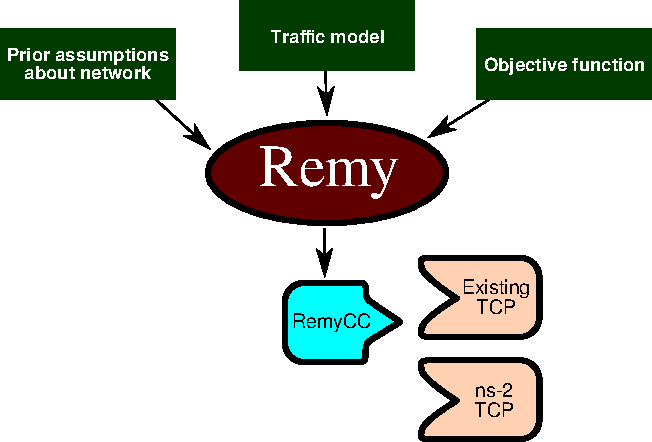
\includegraphics[scale=.6]{remy.pdf}

\end{centering}

\end{frame}

\begin{frame}
\frametitle{Prior knowledge}

\begin{itemize}

\item Uncertain, stochastic model for the network

\begin{itemize}
\item Link speed distribution
\item Delay distribution

\end{itemize}

\item Traffic model

\begin{itemize}
\item ``Conversation''-like (time-based)
\item Datacenter-like workload
\item Web browsing
\end{itemize}

\end{itemize}

\end{frame}

\begin{frame}
\frametitle{Objective function}

\begin{itemize}

\item Tradeoff between \textbf{throughput} and \textbf{delay}

\item Tradeoff between \textbf{efficiency} and \textbf{fairness}

\item Pareto-efficiency

\end{itemize}

\end{frame}

\begin{frame}
\frametitle{Alpha-fairness}

$$U_{\alpha}(x) = \frac{x^{1-\alpha}}{1-\alpha}$$

\begin{itemize}

\item ``Most fair'' Pareto-efficient utility function

\item $\alpha = 0$: efficiency only

\item $\alpha = 2$: min.~potential delay fairness

\item $\alpha \rightarrow \infty$: maximin fairness

\item $\alpha \rightarrow 1$: proportional fairness ($\log(x)$)

\end{itemize}

\end{frame}

\begin{frame}
\frametitle{Objective}

$$\log(\textrm{throughput}) - \delta \log(\textrm{delay})$$

Other options:

\begin{itemize}

\item average flow completion time

\item average transaction completion time

\item 95th percentile transaction completion time

\item \ldots

\end{itemize}

\end{frame}

\begin{frame}
\frametitle{What is this problem?}

\begin{itemize}

\item Decentralized end-to-end algorithm

\item Routing is fixed

\item Each sender only gets its own receiver's acknowledgements

\item Decentralized partially-observable Markov decision process

\item[] (Dec-POMDP)

\end{itemize}

\end{frame}

\begin{frame}
\frametitle{Optimal solution is intractable}

Arbitrary algorithm relates:

\begin{itemize}

\item Full history of acknowledgements

\item Full history of packets sent

\end{itemize}

\ldots to decision about when to send the next packet.

\ssline

Search for algorithm is \textsc{nexp}-complete.

\end{frame}

\begin{frame}
\frametitle{Simplifying the state}

Instead, keep limited state variables:

\begin{enumerate}

\item Moving average of interval between acknowledgements

\item Moving average of interval between sender timestamps reflected in acks

\item Ratio of latest RTT to smallest RTT seen so far

\end{enumerate}

\end{frame}

\begin{frame}
\frametitle{Why these three signals?}

\begin{itemize}

\item More signals increase search time.

\item We explored long-term averages, RTT, etc., but didn't help.

\item Other signals might help other networks!

\item Benefit can be measured empirically.

\end{itemize}

\end{frame}

\begin{frame}
\frametitle{The action}

\begin{enumerate}

\item Increment to congestion window

\item Multiple to congestion window

\item Upper bound on rate of sending

\end{enumerate}

\end{frame}

\begin{frame}
\frametitle{Remy's job}

Rules relate sections of state space to actions.

\begin{quote}
The task: find best set of rules to maximize expected value of
objective function.

\end{quote}

\end{frame}

\begin{frame}
\frametitle{The algorithm (illustration TKTKTKTK)}

\begin{itemize}
\item Initially: one default rule for whole state space

\item Find best action for whole state space

\item Subdivide rule at median query $\rightarrow$ 8 new rules

\item Repeat

\end{itemize}

\ssline

Optimize existing rules and rule structure \textbf{in parallel}.

\end{frame}

\begin{frame}
\frametitle{Fixed 15 Mbps link, 8 senders, flows exp-distributed}

\noindent 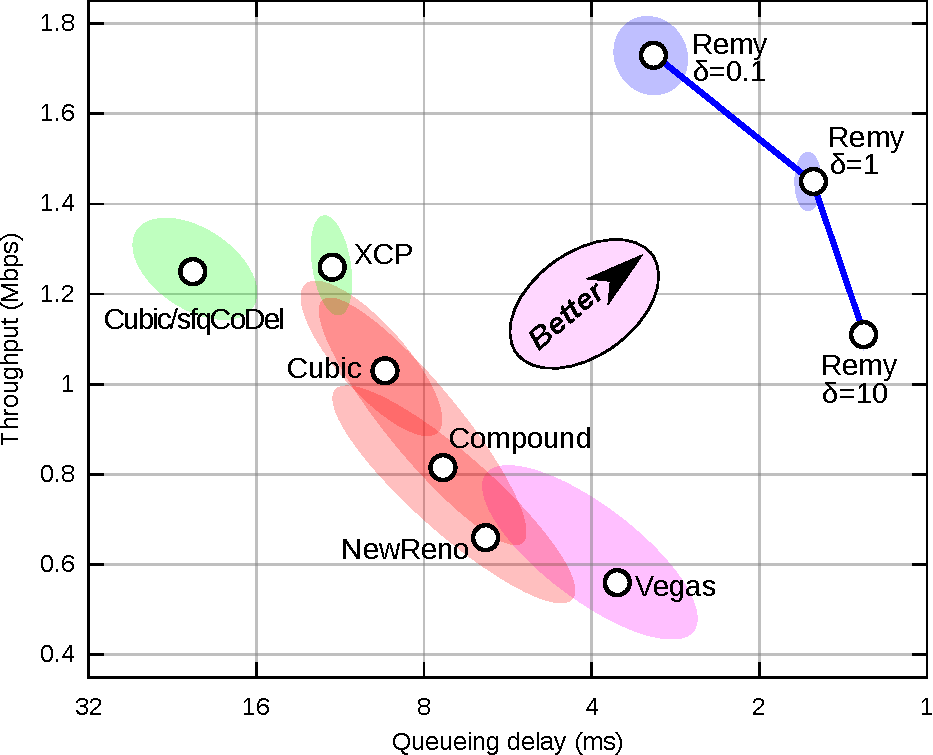
\includegraphics[width=8.5 cm]{eth8-final-bytes.pdf}

\end{frame}

\begin{frame}

\noindent 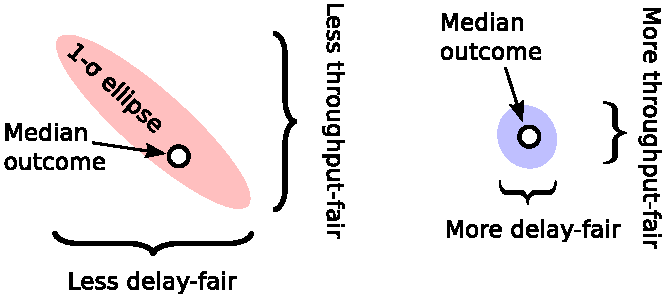
\includegraphics[width=8.5 cm]{legend.pdf}

\end{frame}

\begin{frame}
\frametitle{Fixed 15 Mbps link, 12 senders, heavy-tailed flows}

\noindent 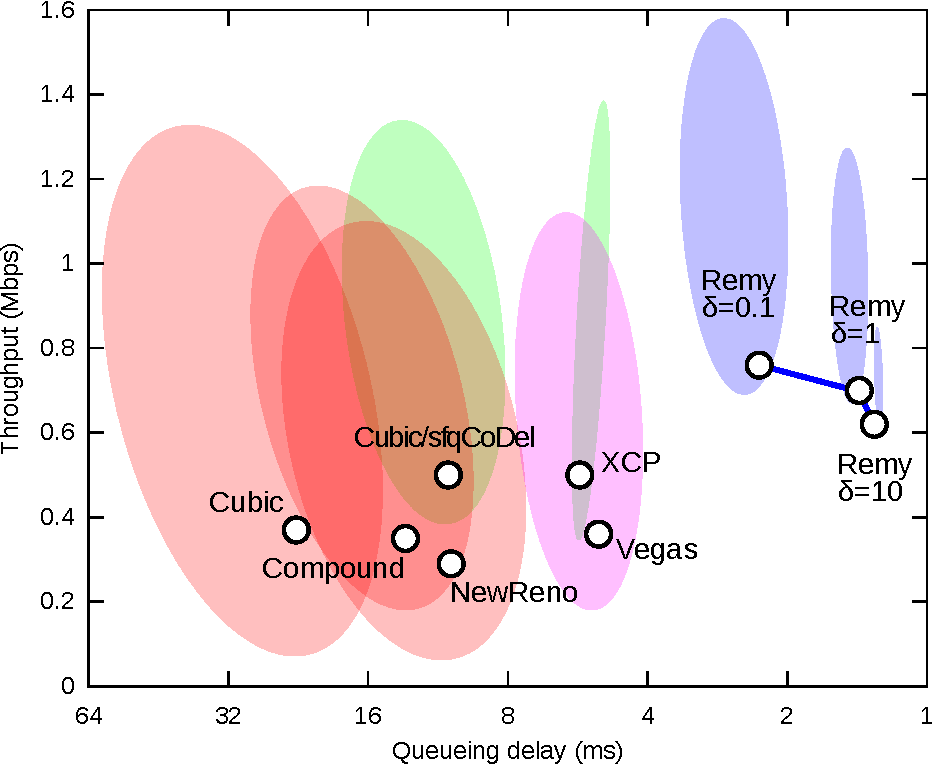
\includegraphics[width=8.5 cm]{eth12-final-flowcdf.pdf}

\end{frame}

\begin{frame}
\frametitle{Verizon LTE, 8 senders, flows exp-distributed}

\noindent 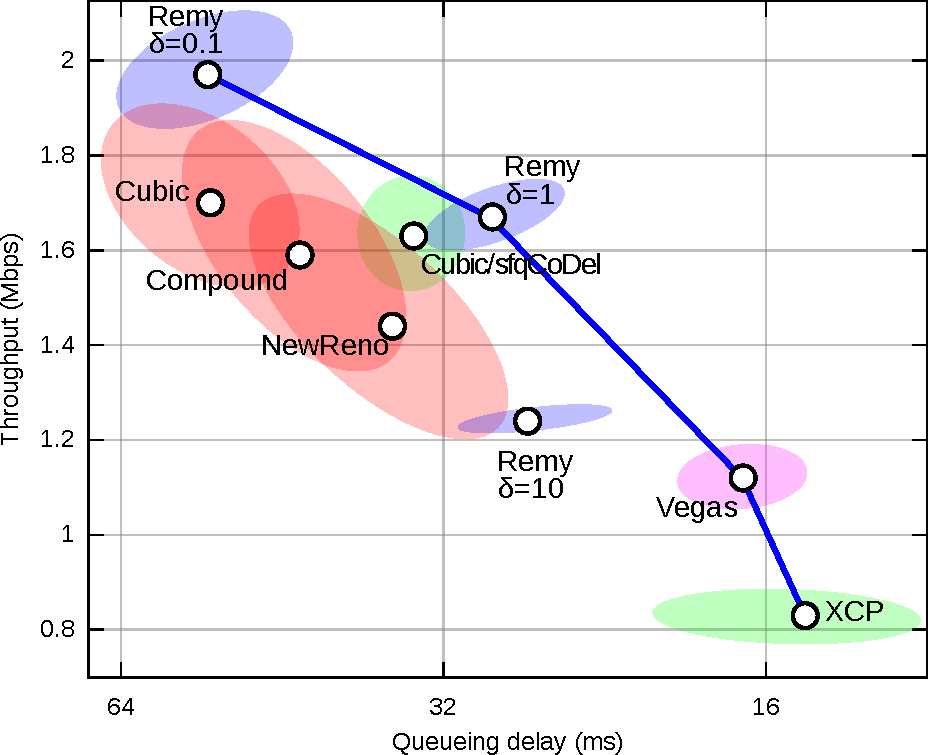
\includegraphics[width=8.5 cm]{vzw-8-final.pdf}

\end{frame}

\begin{frame}
\frametitle{Prior knowledge is helpful, when correct}

\noindent 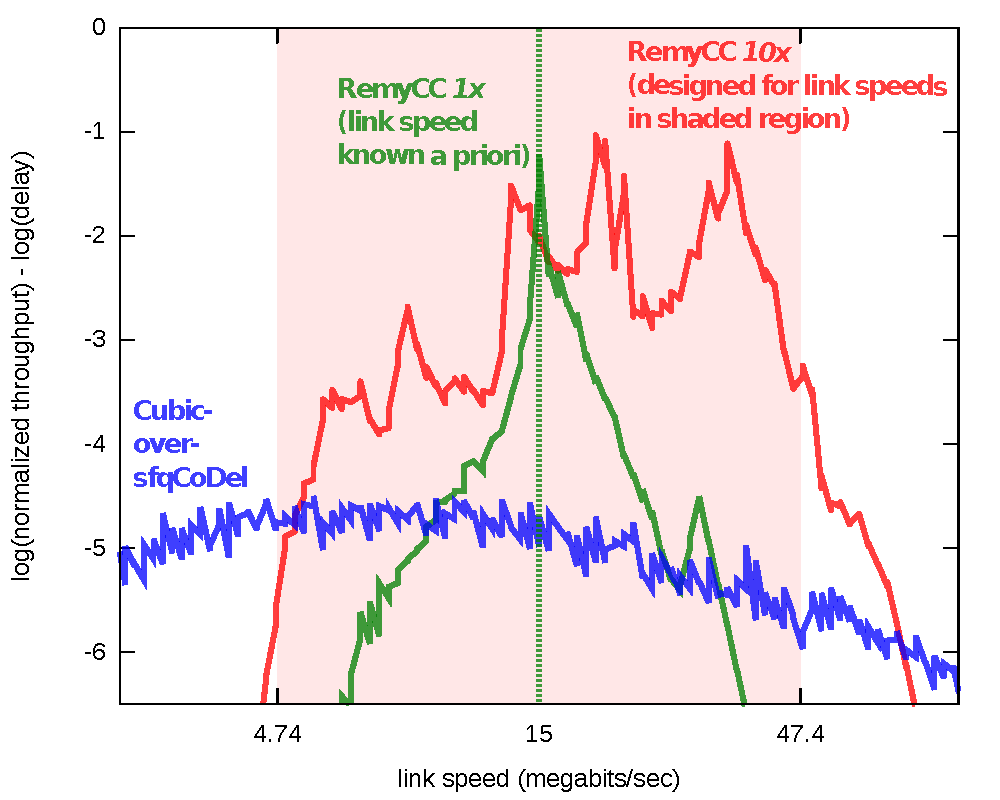
\includegraphics[width=8.5 cm]{spec2.pdf}

\end{frame}

\begin{frame}
\frametitle{Why does Remy work? TKTKTKTKTK}

\begin{itemize}
\item Not entirely clear! (TKTKTKTK)

\item Need to reverse-engineer algorithms.

\item Hundreds of rules --- are they all necessary?
\end{itemize}

\end{frame}

\begin{frame}
\frametitle{Goal-driven algorithm \textbf{moves} the complexity}

\textbf{Human-designed algorithm:}

\begin{itemize}
\item Simple algorithm
\item Complex and subpar emergent behavior
\item \ldots worse when implicit assumptions not met
\end{itemize}

\textbf{Computer-designed algorithm:}

\begin{itemize}
\item Complex algorithm
\item Consistent and good emergent behavior
\item \ldots much worse when stated assumptions not met
\end{itemize}

\end{frame}

\begin{frame}
\frametitle{Evolvability}

\textbf{Status quo:}

\begin{itemize}

\item link layer constrained by need for TCP to perform
\item apps add hacks to get around TCP

\end{itemize}

\textbf{Evolvable transport:}

\begin{itemize}

\item accommodate whatever link layer does \& app wants

\end{itemize}

\end{frame}

\section{}

\begin{frame}
\frametitle{Conclusions}

\begin{itemize}

\item Computer-designed $>$ human-designed

\item End-to-end $>$ in-network

\item Focus on goal and assumptions $>$ focus on mechanism

\end{itemize}

\end{frame}

\begin{frame}
\frametitle{Summary}

\begin{itemize}

\item Find the best schemes for \textbf{evolving} networks and apps.

\item Transport should adapt to what lower layers do \& users want.

\item Focus on policy, not mechanism.

\item Get explicit about assumptions.

\end{itemize}

\ssline

\begin{centering}

http://web.mit.edu/remy

\{keithw,hari\}@mit.edu

\end{centering}

\end{frame}

\end{document}
